%% Преамбула TeX-файла

% 1. Стиль и язык
\documentclass[utf8x, 14pt]{G7-32} % Стиль (по умолчанию будет 14pt)

% Остальные стандартные настройки убраны в preamble.inc.tex.
\sloppy

% Настройки стиля ГОСТ 7-32
% Для начала определяем, хотим мы или нет, чтобы рисунки и таблицы нумеровались в пределах раздела, или нам нужна сквозная нумерация.
%\EqInChapter % формулы будут нумероваться в пределах раздела
%\TableInChapter % таблицы будут нумероваться в пределах раздела
%\PicInChapter % рисунки будут нумероваться в пределах раздела

% Добавляем гипертекстовое оглавление в PDF
\usepackage[
bookmarks=true, colorlinks=true, unicode=true,
urlcolor=black,linkcolor=black, anchorcolor=black,
citecolor=black, menucolor=black, filecolor=black,
]{hyperref}

\AfterHyperrefFix

\usepackage{microtype}% полезный пакет для микротипографии, увы под xelatex мало чего умеет, но под pdflatex хорошо улучшает читаемость

% Тире могут быть невидимы в Adobe Reader
\ifInvisibleDashes
\MakeDashesBold
\fi

\usepackage{graphicx}   % Пакет для включения рисунков

% С такими оно полями оно работает по-умолчанию:
% \RequirePackage[left=20mm,right=10mm,top=20mm,bottom=20mm,headsep=0pt,includefoot]{geometry}
% Если вас тошнит от поля в 10мм --- увеличивайте до 20-ти, ну и про переплёт не забывайте:
\geometry{right=15mm}
\geometry{left=30mm}
\geometry{bottom=20mm}
\geometry{ignorefoot}% считать от нижней границы текста


% Пакет Tikz
\usepackage{tikz}
\usetikzlibrary{arrows,positioning,shadows}

% Произвольная нумерация списков.
\usepackage{enumerate}

% ячейки в несколько строчек
\usepackage{multirow}

% itemize внутри tabular
\usepackage{paralist,array}

%\setlength{\parskip}{1ex plus0.5ex minus0.5ex} % разрыв между абзацами
\setlength{\parskip}{1ex} % разрыв между абзацами
\usepackage{blindtext}

% Центрирование подписей к плавающим окружениям
%\usepackage[justification=centering]{caption}

\usepackage{newfloat}
\DeclareFloatingEnvironment[
placement={!ht},
name=Equation
]{eqndescNoIndent}
\edef\fixEqndesc{\noexpand\setlength{\noexpand\parindent}{\the\parindent}\noexpand\setlength{\noexpand\parskip}{\the\parskip}}
\newenvironment{eqndesc}[1][!ht]{%
    \begin{eqndescNoIndent}[#1]%
\fixEqndesc%
}
{\end{eqndescNoIndent}}




% Настройки листингов.
\ifPDFTeX
% 8 Листинги

\usepackage{listings}

% Значения по умолчанию
\lstset{
  basicstyle= \footnotesize,
  breakatwhitespace=true,% разрыв строк только на whitespacce
  breaklines=true,       % переносить длинные строки
%   captionpos=b,          % подписи снизу -- вроде не надо
  inputencoding=koi8-r,
  numbers=left,          % нумерация слева
  numberstyle=\footnotesize,
  showspaces=false,      % показывать пробелы подчеркиваниями -- идиотизм 70-х годов
  showstringspaces=false,
  showtabs=false,        % и табы тоже
  stepnumber=1,
  tabsize=4,              % кому нужны табы по 8 символов?
  frame=single
}

% Стиль для псевдокода: строчки обычно короткие, поэтому размер шрифта побольше
\lstdefinestyle{pseudocode}{
  basicstyle=\small,
  keywordstyle=\color{black}\bfseries\underbar,
  language=Pseudocode,
  numberstyle=\footnotesize,
  commentstyle=\footnotesize\it
}

% Стиль для обычного кода: маленький шрифт
\lstdefinestyle{realcode}{
  basicstyle=\scriptsize,
  numberstyle=\footnotesize
}

% Стиль для коротких кусков обычного кода: средний шрифт
\lstdefinestyle{simplecode}{
  basicstyle=\footnotesize,
  numberstyle=\footnotesize
}

% Стиль для BNF
\lstdefinestyle{grammar}{
  basicstyle=\footnotesize,
  numberstyle=\footnotesize,
  stringstyle=\bfseries\ttfamily,
  language=BNF
}

% Определим свой язык для написания псевдокодов на основе Python
\lstdefinelanguage[]{Pseudocode}[]{Python}{
  morekeywords={each,empty,wait,do},% ключевые слова добавлять сюда
  morecomment=[s]{\{}{\}},% комменты {а-ля Pascal} смотрятся нагляднее
  literate=% а сюда добавлять операторы, которые хотите отображать как мат. символы
    {->}{\ensuremath{$\rightarrow$}~}2%
    {<-}{\ensuremath{$\leftarrow$}~}2%
    {:=}{\ensuremath{$\leftarrow$}~}2%
    {<--}{\ensuremath{$\Longleftarrow$}~}2%
}[keywords,comments]

% Свой язык для задания грамматик в BNF
\lstdefinelanguage[]{BNF}[]{}{
  morekeywords={},
  morecomment=[s]{@}{@},
  morestring=[b]",%
  literate=%
    {->}{\ensuremath{$\rightarrow$}~}2%
    {*}{\ensuremath{$^*$}~}2%
    {+}{\ensuremath{$^+$}~}2%
    {|}{\ensuremath{$|$}~}2%
}[keywords,comments,strings]

% Подписи к листингам на русском языке.
\renewcommand\lstlistingname{Листинг}
\renewcommand\lstlistlistingname{Листинги}

\else
\usepackage{local-minted}
\fi

% Полезные макросы листингов.
% Любимые команды
\newcommand{\Code}[1]{\textbf{#1}}


% Стиль титульного листа и заголовки

%\NirEkz{Экз. 3}                                  % Раскоментировать если не требуется
%\NirGrif{Секретно}                % Наименование грифа

%\gosttitle{Gost7-32}       % Шаблон титульной страницы, по умолчанию будет ГОСТ 7.32-2001, 
% Варианты GostRV15-110 или Gost7-32 
 
\NirOrgLongName{Министерство общего и профессионального образования \\
Российской Федерации\par
УФИМСКИЙ ГОСУДАРСТВЕННЫЙ АВИАЦИОННЫЙ ТЕХНИЧЕСКИИ УНИВЕРСИТЕТ
}                                           %% Полное название организации

\NirUdk{УДК № 378.14}
\NirGosNo{№ госрегистрации 01970006723}
%\NirInventarNo{Инв. № ??????}

%\NirConfirm{Согласовано}                  % Смена УТВЕРЖДАЮ
\NirBoss[.49]{Проректор университета\\по научной работе}{Н.С. Жернаков}            %% Заказчик, утверждающий НИР


%\NirReportName{Научно-технический отчет}   % Можно поменять тип отчета
%\NirAbout{О составной части \par опытно-конструкторской работы} %Можно изменить о чем отчет

%\NirPartNum{Часть}{1}                      % Часть номер

%\NirBareSubject{}                  % Убирает по теме если раскоментить

% \NirIsAnnotacion{АННОТАЦИОННЫЙ }         %% Раскомментируйте, если это аннотационный отчёт
%\NirStage{промежуточный}{Этап \No 1}{} %%% Этап НИР: {номер этапа}{вид отчёта - промежуточный или заключительный}{название этапа}
%\NirStage{}{}{} %%% Этап НИР: {номер этапа}{вид отчёта - промежуточный или 

\Nir{Социально-экономические проблемы подготовки военных специалистов\\в гражданских вузах России}

\NirSubject{ФЕМИНИЗАЦИЯ АРМИИ КАК СОЦИАЛЬНЫЙ ПРОЦЕСС  }                                   % Наименование темы
%\NirFinal{}                        % Заключительный, если закоментировать то промежуточный
%\finalname{итоговый}               % Название финального отчета (Заключительный) 
%\NirCode{Шифр\,---\,САПР-РЛС-ФИЗТЕХ-1} % Можно задать шифр как в ГОСТ 15.110
\NirCode{}

\NirManager{Зам. проректора по научной работе}{Р.А. Бадамшин  } %% Название руководителя
\NirIsp{Руководитель темы}{Г.А. Кабакович} %% Название руководителя

\NirYear{1999}%% если нужно поменять год отчёта; если закомментировано, ставится текущий год
\NirTown{Уфа}                           %% город, в котором написан отчёт



\begin{document}

\frontmatter % выключает нумерацию ВСЕГО; здесь начинаются ненумерованные главы: реферат, введение, глоссарий, сокращения и прочее.

\maketitle %создает титульную страницу


\begin{executors}
\personalSignature{Первый исполнитель}{ФИО}

\personalSignature{Второй исполнитель}{ФИО}
\end{executors}


%\listoffigures                         % Список рисунков

%\listoftables                          % Список таблиц

%\NormRefs % Нормативные ссылки 
% Команды \breakingbeforechapters и \nonbreakingbeforechapters
% управляют разрывом страницы перед главами.
% По-умолчанию страница разрывается.

% \nobreakingbeforechapters
% \breakingbeforechapters

% Также можно использовать \Referat, как в оригинале
\begin{abstract}

    Отчет содержит \pageref{LastPage}\,стр.%
    \ifnum \totfig >0
    , \totfig~рис.%
    \fi
    \ifnum \tottab >0
    , \tottab~табл.%
    \fi
    %
    \ifnum \totbib >0
    , \totbib~источн.%
    \fi
    %
    \ifnum \totapp >0
    , \totapp~прил.%
    \else
    .%
    \fi
\end{abstract}

%%% Local Variables: 
%%% mode: latex
%%% TeX-master: "rpz"
%%% End: 


\tableofcontents

\printnomenclature % Автоматический список сокращений

\Introduction

Сервис для агрегирования инфомарции по call-центру предназначен для наблюдения за различными актуальными
показателями работы call-центра.

Многим супервизорам или руководителям отделов требуется, время от времени, знать,
что происходит в call-центре, в каком состоянии находятся операторы, проекты или звонки.
Это знание поможет им принять правильное решение, учитывающее текущую обстановку, например,
так они смогут в случае, если нагрузка на какой-то конкретный проект сильно возросла
и операторы не справляются с поступающими вызовами,
перевести больше операторов на проект или перераспределить вызовы на другие проекты.
Разрабатываемый сервис предназначен решить проблему наблюдения в удобной форме,
предоставляя различные сводки и временные графики.

\Define{Naumen Contact Center}{полнофункциональное программное решение для построения крупных и средних контактных центров} %todo [https://www.naumen.ru/products/phone/]
\Define{Naumen}{российская компания, разработчик программного обеспечения, основана в 2001 году в Екатеринбурге}
Сервис будет использоваться и распространяться в составе программного продукта Naumen Contact Center.
Naumen Contact Center (ранее Naumen Phone) разрабатывается российской компанией Naumen.
Проектный офис и внедренческий центр компании находится в Москве, разработка ведётся в Екатеринбурге, Твери, Челябинске,
Санкт-Петербурге и Севастополе.
В компании действует собственный учебный и сервисный центр.
Существует дочерняя компания в Казахстане, занимающаяся работой с клиентами из Средней Азии.
В состав NCC входит коммуникационная платформа с компонентом Omni-Channel, WFM
\Abbrev{WFM}{информационная система управления проектами и прогнозирования рабочей нагрузки},
а также автоматизированные рабочие места оператора и супервизора.
Клиентами Naumen являются:
ИнтерРАО
ЕС,
Спортмастер,
Банк
Россия,
Мосэнергосбыт,
Moldtelecom.
Платформа Naumen Contact Center включена в глобальный отчет Gartner.

На текущий момент на рынке представлено достаточное количество решений для реализации наблюдения за работой call-центра.
Но все они, либо являются частью конкурирующих программный продуктов для автоматизации call-центров,
либо интеграция с ними является не тривиальной задачей,
т.~к. для реализации наблюдения за состоянием call-центра нужно учитывать многие внутренние механизмы и протоколы.
Поэтому было решено разработать собственное решение, которое учитывало бы все ньюансы работы внутри NCC.
\Abbrev{NCC}{Naumen Contact Center}

Это уже не первая попытка реализации сервиса такого рода.
Предыдущая попытка закончилась с переменным успехом: сервис не обеспечивал достаточный уровень актуальности данных
на call-центрах с больших количеством операторов.
Поэтому, в случае успеха, от него планируется отказаться.

Главным аргументом успешности текущей реализации является изменение технологического стека,
если предыдущие попытки были реализованы с помощью языка Python 2.7 и сетевого движка Twisted, %todo [https://twistedmatrix.com/trac/]
то текущая попытка реализации будет выполнена на языке Go.
Go предоставляет средства и возможности для разработки производительного сетевого микросервиса.





\mainmatter % это включает нумерацию глав и секций в документе ниже

\chapter{Постановка задачи}
\label{cha:analysis}
%
% % В начале раздела  можно напомнить его цель
%

\section{Описание объекта автоматизации}

\subsection{Краткие сведения об объекте автоматизации}

\Abbrev{RRS}{Real-time report subsystem --- подсистема отчетов реального времени}
Объектом автоматизации сервиса для агрегирования информации по call-центру (далее RRS) является часть обязанностей супервизора,
связанных с наблюдением за текущим состоянием доверенных ему проектов и операторов.

\subsection{Сведения об условиях эксплуатации объекта автоматизации}

RRS является частью Naumen Contact Center.
NCC состоит из модулей и сервисов, каждый из которых выполняет свою функцию.
Обмен данными между компонентами NCC осуществляется по стандартным сетевым протоколам,
что позволяет физически размещать компоненты продукта на разных серверах.
Такая особенность архитектуры позволяет строить масштабируемые call-центры
для одновременного обслуживания массового количества вызовов.

NCC позволяет решать следующие основные задачи:
\begin{itemize}
    \item организация проектов по обработке входящих обращений, в том числе:
        \begin{itemize}
            \item обработка потока входящих телефонных вызовов;
            \item обработка потока входящих E-mail-сообщений;
            \item обработка потока входящих SMS-сообщений;
            \item обработка входящих мгновенных сообщений;
        \end{itemize}
    \item организация исходящих проектов, включая:
        \begin{itemize}
            \item автоматические исходящие обзвоны;
            \item E-mail рассылки;
        \end{itemize}
    \item организация смешанных проектов, включая:
        \begin{itemize}
            \item обработка обращений, поступивших по различным каналам связи одним и тем же оператором;
            \item обработка как входящих обращений, так и исходящих вызовов одним и тем же оператором;
        \end{itemize}
    \item контроль работы операторов, в том числе:
        \begin{itemize}
            \item осуществление записи разговоров;
            \item получение отчетности;
            \item управление качеством обработки вызовов.
        \end{itemize}
\end{itemize}

\Abbrev{PMS}{Project Management System --- система управления проектами}
Система управления проектами (PMS) представляет собой Web-ориентированную систему
управления проектами по обслуживанию обращений клиентов.
PMS включает в себя следующие основные функции:
\begin{itemize}
    \item управление партнерами, которые выступают в качестве заказчиков на проекты по обслуживанию вызовов;
    \item формирование и ведение проектов, в том числе:
        \begin{itemize}
            \item формирование состава участников;
            \item разработка сценариев обслуживания обращений;
            \item формирование заданий на обслуживание вызовов;
            \item контроль хода выполнения работ по проекту;
        \end{itemize}
    \item использование встроенного программного телефона WebPhone;
    \item формирование отчетности и предоставление ее партнерам.
\end{itemize}

\Define{NauCore}{Сервис шины управляющих сообщений, обеспечивает работу остальных сервисов NCC и их взаимодействие между собой}
PMS взаимодействует с другими сервисами через брокер сообщений NauCore посредством внутреннего протокола обмена сообщениям NCC.

NauCore запускается при загрузке операционной системы и выполняет следующие функции:
\begin{itemize}
    \item осуществляет взаимодействие других компонентов NCC между собой;
    \item автоматически запускает и контролирует работу других телефонных сервисов. При аварийном завершении работы какого-либо сервиса пытается его перезапустить;
    \item предоставляет интерфейс управления сервисами, которые он контролирует:
        \begin{itemize}
            \item web-интерфейс;
            \item командная строка;
        \end{itemize}
    \item осуществляет ротацию журналов работы сервисов.
\end{itemize}

Сервисы NauCore устанавливаются на каждый сервер NCC,
соединяются между собой и образуют общую шину обмена сообщениями.
При запуске каждый сервис NauCore автоматически запускает другие сервисы NCC
и обеспечивает их взаимодействие через общую шину.

NCC использует для связи компонент системы XML-over-TCP протокол.

\Abbrev{СУБД}{система управления базой данных}
\Define{PostgreSQL}{свободная объектно-реляционная система управления базами данных}
\Define{Oracle DB или Oracle RDBMS}{объектно-реляционная~система управления базами данных компании Oracle}
NCC в качестве базы данных использует общую СУБД, которой может быть либо PostgreSQL, либо Oracle DB.

RRS проектируется как отдельный сервис в NCC,
при этом задачу отображения данных берет на себя NCC PMS,
а сами данные нужно будет получать из NauCore\cite{Pup09}. %todo убрать

\chapter{Конструкторский раздел}
\label{cha:design}

В данном разделе проектируется новая всячина.

\section{Архитектура всячины}

\subsection{Протестируем подпункт}
\subsubsection{А теперь подподпункт}


\paragraph{Проверка} параграфа. Вроде работает.
\paragraph{Вторая проверка} параграфа. Опять работает.

Вот.

\begin{itemize}
\item Это список с <<палочками>>.
\item Хотя он и по ГОСТ, но\dots
\end{itemize}

\begin{enumerate}
\item  Для списка, начинающегося с заглавной буквы, лучше список с цифрами.
\end{enumerate}

Формула \eqref{F:F1} совершено бессмысленна.

%Кстати, при каких-то условиях <<удавалось>> получить двойный скобки вокруг номеров формул. Вопрос исследуется.

\begin{equation}
a= cb
\label{F:F1}
\end{equation}

А формула~\eqref{eq:fourierrow} имеет некоторый смысл.
Кроме этого она пытается иллюстрировать применение окружения \Code{eqndesc} которое размещает формулу совместно с её описанием.
Однако обратите внимание на нумерацию формул~\eqref{eq:fourierrow} и \eqref{F:F2}, попробуйте добавить \Code{[H]} к такой формуле.

\begin{eqndesc}
    \begin{equation}\label{eq:fourierrow}
        f(x) = \frac{a_0}{2} + \sum\limits_{k=1}^{+\infty} A_k\cos\left(k\frac{2\pi}{\tau}x+\theta_k\right)
    \end{equation}

    где $A_k$ "--- амплитуда  k-го гармонического колебания,\\
    $A_k$ "--- амплитуда $k$-го гармонического колебания,\\
    $ k\frac{2\pi}{\tau} = k\omega$ "--- круговая частота гармонического колебания,\\
    $\theta_k$ "--- начальная фаза $k$-го колебания.
\end{eqndesc}


Окружение \texttt{cases} опять работает (см. \eqref{F:F2}), спасибо И. Короткову за исправления..


\begin{equation}
a= \begin{cases}
 3x + 5y + z, \mbox{если хорошо} \\
 7x - 2y + 4z, \mbox{если плохо}\\
 -6x + 3y + 2z, \mbox{если совсем плохо}
\end{cases}
\label{F:F2}
\end{equation}

\section{Подсистема всякой ерунды}

Культурная вставка dot-файлов через утилиту dot2tex (рис.~\ref{fig:fig02}).

\begin{figure}
  \centering
% [width=0.5\textwidth] --- регулировка ширины картинки
  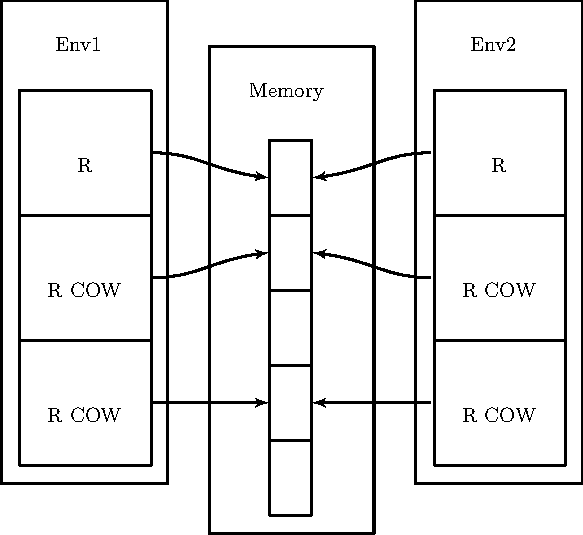
\includegraphics[width=.5\textwidth]{inc/dot/cow2}
  \caption{Рисунок}
  \label{fig:fig02}
\end{figure}


\subsection{Блок-схема всякой ерунды}

\subsubsection*{Кстати о заголовках}

У нас есть и \Code{subsubsection}. Только лучше её не нумеровать.

%%% Local Variables:
%%% mode: latex
%%% TeX-master: "rpz"
%%% End:

\chapter{Технологический раздел}
\label{cha:impl}

В данном разделе описано изготовление и требование всячины. Кстати,
в Latex нужно эскейпить подчёркивание (писать <<\verb|some\_function|>> для \Code{some\_function}).

\ifPDFTeX
Для вставки кода есть пакет \Code{listings}. К сожалению, пакет \Code{listings} всё ещё
работает криво при появлении в листинге русских букв и кодировке исходников utf-8.
В данном примере он (увы) на лету конвертируется в koi-8 в ходе сборки pdf.

Есть альтернатива \Code{listingsutf8}, однако она работает лишь с
\Code{\textbackslash{}lstinputlisting}, но не с окружением \Code{\textbackslash{}lstlisting}

Вот так можно вставлять псевдокод (питоноподобный язык определен в \Code{listings.inc.tex}):

\begin{lstlisting}[style=pseudocode,caption={Алгоритм оценки дипломных работ}]
def EvaluateDiplomas():
    for each student in Masters:
        student.Mark := 5
    for each student in Engineers:
        if Good(student):
            student.Mark := 5
        else:
            student.Mark := 4
\end{lstlisting}

Еще в шаблоне определен псевдоязык для BNF:

\begin{lstlisting}[style=grammar,basicstyle=\small,caption={Грамматика}]
  ifstmt -> "if" "(" expression ")" stmt |
            "if" "(" expression ")" stmt1 "else" stmt2
  number -> digit digit*
\end{lstlisting}

В листинге~\ref{lst:sample01} работают русские буквы. Сильная магия. Однако, работает
только во включаемых файлах, прямо в \TeX{} нельзя.

% Обратите внимание, что включается не ../src/..., а inc/src/...
% В Makefile есть соответствующее правило для inc/src/*,
% которое копирует исходные файлы из ../src и конвертирует из UTF-8 в KOI8-R.
% Кстати, поэтому использовать можно только русские буквы и ASCII,
% весь остальной UTF-8 вроде CJK и египетских иероглифов -- нельзя.

\lstinputlisting[language=C,caption=Пример (\Code{test.c}),label=lst:sample01]{inc/src/test.c}

\else

Для вставки кода есть пакет \texttt{minted}. Он хорош всем кроме: необходимости Python (есть во всех нормальных (нет, Windows, я не про тебя) ОС) и Pygments и того, что нормально работает лишь в \XeLaTeX.

\ifdefined\NoMinted
Но к сожалению, у вас, по-видимому, не установлен Python или pygmentize.
\else
Можно пользоваться расширенным BFN:

\begin{listing}[H]
\begin{ebnfcode}
 letter = "A" | "B" | "C" | "D" | "E" | "F" | "G"
       | "H" | "I" | "J" | "K" | "L" | "M" | "N"
       | "O" | "P" | "Q" | "R" | "S" | "T" | "U"
       | "V" | "W" | "X" | "Y" | "Z" ;
digit = "0" | "1" | "2" | "3" | "4" | "5" | "6" | "7" | "8" | "9" ;
symbol = "[" | "]" | "{" | "}" | "(" | ")" | "<" | ">"
       | "'" | '"' | "=" | "|" | "." | "," | ";" ;
character = letter | digit | symbol | "_" ;
 
identifier = letter , { letter | digit | "_" } ;
terminal = "'" , character , { character } , "'" 
         | '"' , character , { character } , '"' ;
 
lhs = identifier ;
rhs = identifier
     | terminal
     | "[" , rhs , "]"
     | "{" , rhs , "}"
     | "(" , rhs , ")"
     | rhs , "|" , rhs
     | rhs , "," , rhs ;
 
rule = lhs , "=" , rhs , ";" ;
grammar = { rule } ;
\end{ebnfcode}
\caption{EBNF определённый через EBNF}
\label{lst:ebnf}
\end{listing}

А вот в листинге \ref{lst:c} на языке C работают русские комменты. Спасибо Pygments и Minted за это.

\begin{listing}[H]
\cfile{inc/src/test.c}
\caption{Пример — test.c} 
\end{listing}
\label{lst:c}

\fi
\fi
% Для вставки реального кода лучше использовать \texttt{\textbackslash lstinputlisting} (который понимает
% UTF8) и стили \Code{realcode} либо \Code{simplecode} (в зависимости от размера куска).




Можно также использовать окружение \Code{verbatim}, если \Code{listings} чем-то не
устраивает. Только следует помнить, что табы в нём <<съедаются>>. Существует так же команда \Code{\textbackslash{}verbatiminput} для вставки файла.

\begin{verbatim}
a_b = a + b; // русский комментарий
if (a_b > 0)
    a_b = 0;
\end{verbatim}

%%% Local Variables:
%%% mode: latex
%%% TeX-master: "rpz"
%%% End:

\chapter{Экспериментальный раздел}
\label{cha:research}

В данном разделе проводятся вычислительные эксперименты.
А на рис.~\ref{fig:spire01} показана схема мыслительного процесса автора...

\begin{figure}
  \centering
  \includegraphics[width=\textwidth]{inc/svg/pic01}
  \caption{Как страшно жить}
  \label{fig:spire01}
\end{figure}


%%% Local Variables:
%%% mode: latex
%%% TeX-master: "rpz"
%%% End:

\chapter{Организационно-экономический раздел}
\label{cha:econom}

\section{Протестируем специальные символы.}

И заодно переключение шрифтов.


{\shorthandoff" \texttt{"-{}-* Прямая речь "-{}-{}- <{}<после ,{},тире`{}` неразрывный пробел>{}>}}

{\cyrillicfonttt{\bfseries\itshape\textbackslash{}cyrillicfonttt}
"--* Прямая речь "--- <<после ,,тире`` неразрывный пробел>>.}

{\cyrillicfontsf{\bfseries\itshape\textbackslash{}cyrillicfontsf}
"--* Прямая речь "--- <<после ,,тире`` неразрывный пробел>>.}

{\cyrillicfont{\bfseries\itshape\textbackslash{}cyrillicfont}
"--* Прямая речь "--- <<после ,,тире`` неразрывный пробел>>.}


\blindtext
%%% Local Variables:
%%% mode: latex
%%% TeX-master: "rpz"
%%% End:

\chapter{Промышленная экология и безопасность}\label{cha:bzd}

\blindtext

\blindlistlist[3]{enumerate}

%%% Local Variables:
%%% mode: latex
%%% TeX-master: "rpz"
%%% End:


\backmatter %% Здесь заканчивается нумерованная часть документа и начинаются ссылки и
            
\Conclusion % заключение к отчёту

В результате проделанной работы стало ясно, что ничего не ясно...

%%% Local Variables: 
%%% mode: latex
%%% TeX-master: "rpz"
%%% End: 
%% заключение


% % Список литературы при помощи BibTeX
% Юзать так:
%
% pdflatex rpz
% bibtex rpz
% pdflatex rpz

\bibliographystyle{ugost2008}
\bibliography{rpz}

%%% Local Variables: 
%%% mode: latex
%%% TeX-master: "rpz"
%%% End: 



\appendix   % Тут идут приложения

\chapter{Картинки}
\label{cha:appendix1}

\blindtext
\begin{figure}
\centering
\caption{Картинка в приложении. Страшная и ужасная.}
\end{figure}

%%% Local Variables: 
%%% mode: latex
%%% TeX-master: "rpz"
%%% End: 


\chapter{Еще картинки}
\label{cha:appendix2}
\blindtext

\begin{figure}
\centering
\caption{Еще одна картинка, ничем не лучше предыдущей. Но надо же как-то заполнить место.}
\end{figure}

%%% Local Variables: 
%%% mode: latex
%%% TeX-master: "rpz"
%%% End: 


\end{document}

%%% Local Variables:
%%% mode: latex
%%% TeX-master: t
%%% End:
